\section{Ergebnisse}
\newpage
\begin{figure}[htbp]
    \centering
        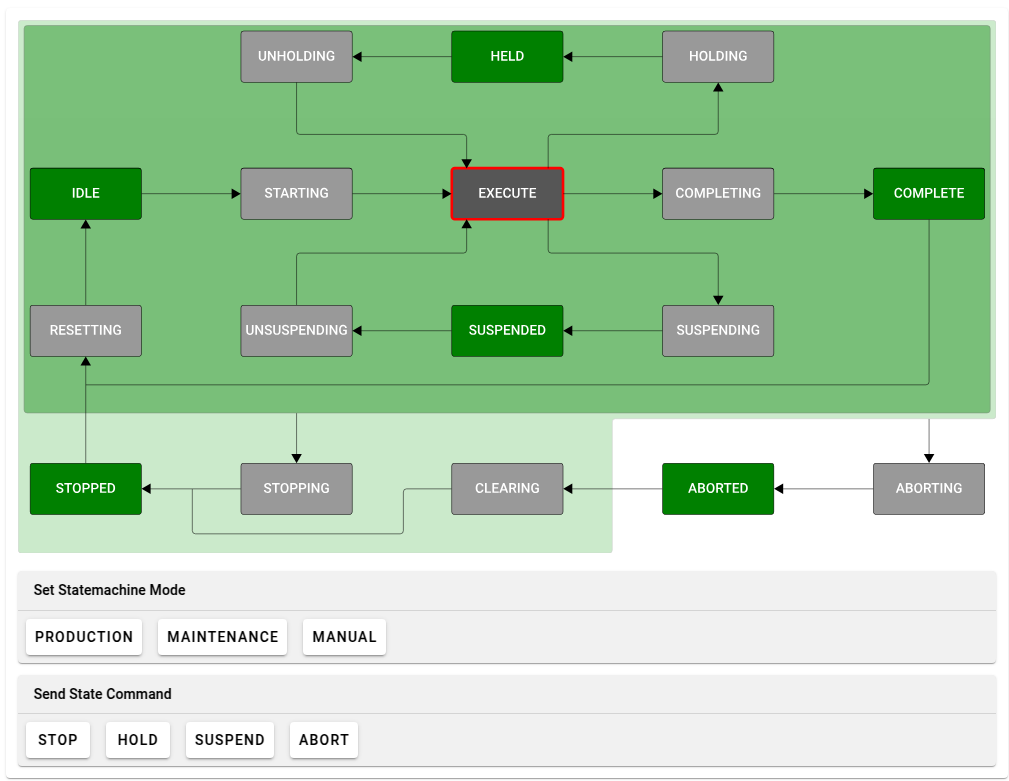
\includegraphics[width=1\textwidth]{Bilder/Ergebnisse/2025-07-23_15-06.png}
    
    \caption{Sequenzdiagramm zur Aggregation des PCF}
    \label{fig:SequenzdiagrammPCF}
\end{figure}

\begin{figure}[htbp]
    \centering
        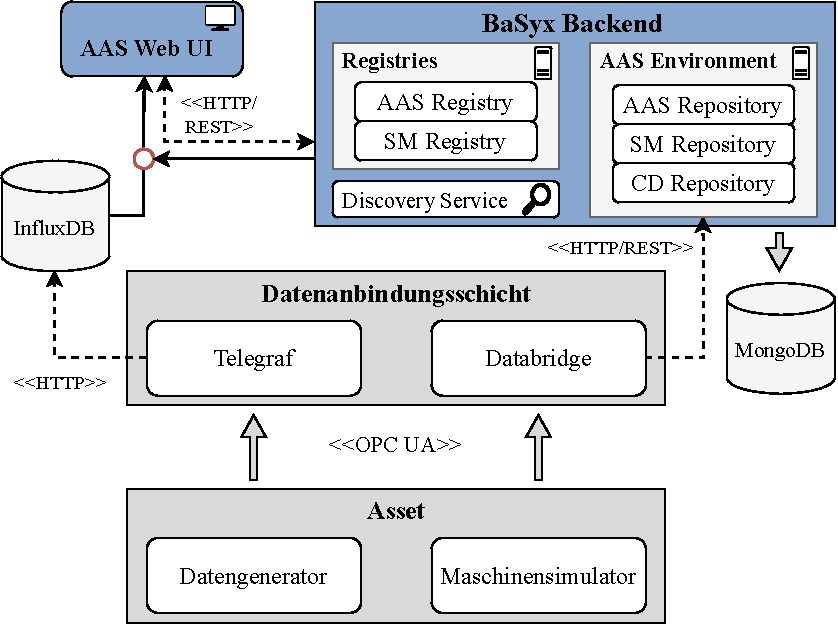
\includegraphics[width=1\textwidth]{Bilder/Ergebnisse/DynamischeDaten/Architektur.pdf}
    
    \caption{Sequenzdiagramm zur Aggregation des PCF}
    \label{fig:SequenzdiagrammPCF}
\end{figure}

%AAS Demonstrator
\subsection{AAS-Demonstrator für die robocell}
\subsubsection{Systemarchitektur}
\subsubsection{Eingesetzte Teilmodelle}
\subsubsection{Herausforderungen bei der Erstellung}

%KI-Modell
\subsection{Evaluation des KI-Modells}
\subsubsection{Bewertung des prototypischen KI-Einsatzes}
\subsubsection{Ausblick: Predictive Maintenance}
\subsubsection{Weiterführende Einsatzmöglichkeiten}

% Digitaler Produktpass
\subsection{Anwendungsfall Digitaler Produktpass}
\subsubsection{Abbildung des PCF}
\subsubsection{Rollenbasierter Zugriff auf Submodelle}

Die beschriebene Lösung ermöglicht es, den \acs{pcf} dynamisch auf Basis der in der Komponentenliste referenzierten Steuerungselemente zu berechnen. 
Auch wenn derzeit nur ausgewählte Komponenten berücksichtigt werden, lässt sich die Liste bei Verfügbarkeit weiterer Komponenten-\acs{aas} unkompliziert erweitern, sodass sukzessive die gesamte Maschine in die Berechnung einbezogen werden kann. 
Perspektivisch lässt sich die Berechnung zudem um weitere Lebenszyklusphasen wie Nutzung oder Entsorgung ergänzen, um eine ganzheitliche Betrachtung von der Herstellung bis zum Lebensende eines Produkts bzw. einer Maschine zu ermöglichen.


PCF
Die entwickelte Lösung konnte erfolgreich demonstrieren, dass eine dynamische Aggregation des \acs{pcf} für ein Anlagenmodul auf Basis verteilter Komponenten-AAS möglich ist. Die über die globalAssetId referenzierten Steuerungskomponenten wurden automatisiert ausgelesen und ihre jeweiligen \acs{pcf}-Werte für die Phasen Material, Produktion sowie Cradle to Gate korrekt ermittelt.

Die ermittelten Einzelwerte wurden aggregiert und als strukturierte CO\textsubscript{2}-Äquivalente zurück in das Carbon Footprint-Submodell der Haupt-AAS geschrieben. Damit steht der aggregierte \acs{pcf} direkt in der AAS der RoboCell zur Verfügung und kann über die AAS Web UI oder andere Dienste weiterverarbeitet werden.

Ein ergänzendes Plugin ermöglicht die interaktive Visualisierung der Werte in der Benutzeroberfläche. Es zeigt die Einzelbeiträge der Komponenten sowie die Gesamtsumme in den jeweiligen Phasen, wodurch eine nachvollziehbare und transparente Darstellung des \acs{pcf} erzielt wird.

Die Lösung wurde mit einer Auswahl realer Siemens-Komponenten erprobt. Auch wenn derzeit nur eine Teilmenge des vollständigen Maschinenaufbaus berücksichtigt wurde, zeigt der Ansatz eine hohe Erweiterbarkeit: Weitere Komponenten-AAS können bei Verfügbarkeit problemlos eingebunden und in die Aggregation integriert werden.

Zugriffsrechte
Zusätzlich wurde die technische Umsetzbarkeit der Zugriffssteuerung im Kontext des digitalen Produktpasses geprüft. Erste Tests zeigen, dass sich differenzierte Zugriffskontrollen auf Submodell-Ebene technisch realisieren lassen. Dies bietet Potenzial für zukünftige Szenarien, bei denen sensible Nachhaltigkeitsdaten nur bestimmten Akteuren entlang der Wertschöpfungskette zugänglich gemacht werden sollen.

\subsection{Anwendungsfall automatisierte Generierung der AAS}
% \subsection{Einsatzmöglichkeiten von KI im Kontext der Verwaltungsschale}
% \subsubsection{Generierung von Verwaltungsschalen}
% \subsubsection{Anomaliererkennung}
% \subsubsection{Weiterführende Einsatzmöglichkeiten}

%Evaluation der eingesetzten Software
\subsection{Evaluierung eingesetzter Tools und Software}
\subsubsection{AASX Package Explorer}
\subsubsection{Eclipse AASX Server}
\subsubsection{BaSyx}
\subsubsection{Mnestix Browser}
Optional davor halt nicht drauf eingeganen\dots